\documentclass[11pt,a4paper]{scrartcl}
\typearea{12}
\usepackage{graphicx}
\usepackage{pstricks}
\usepackage{amsmath}
\begin{document}


\section*{An introduction to programming}

Here is a simple programme for drawing a square; we will start with
this and try to make more complicated drawings.
\begin{center}
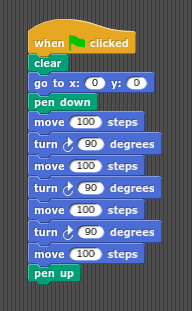
\includegraphics{basic_square.png}
\end{center}
Enter this and make sure it draws a square! One thing about this
program is that after it draws the square the arrow ends up pointing a
different direction to the direction it started in; can you fix this?
\begin{center}
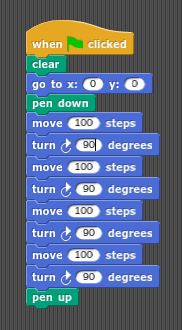
\includegraphics{basic_square_point.png}
\end{center}
Repeat
\begin{center}
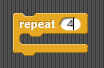
\includegraphics{repeat.png}
\end{center}
Can you use that to make the programme more succinct and readable? 
\begin{center}
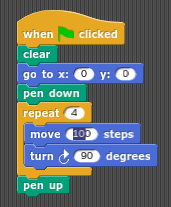
\includegraphics{repeat_square.png}
\end{center}
Can you make a programme to draw something that looks like a circle but going forward a tiny bit and turning again and again?
\begin{center}
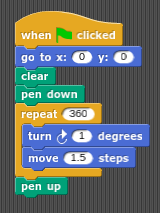
\includegraphics{circle.png}
\end{center}

Now, look at this programme
\begin{center}
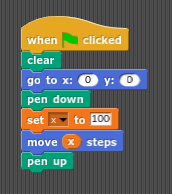
\includegraphics{variable.png}
\end{center}
Do the same to your square programme!
\begin{center}
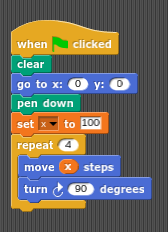
\includegraphics{variable_square.png}
\end{center}


This programme does something slighly more useful with a variable.
\begin{center}
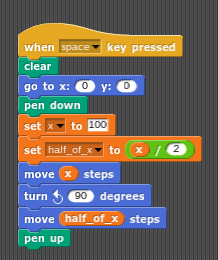
\includegraphics{line_half_line.png}
\end{center}
Try modifying your programme in a similar way so that it draws an
$n$-gon.
\begin{center}
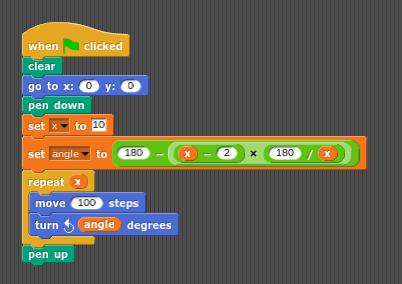
\includegraphics{n_gon.png}
\end{center}


In this programme the variable is changed in the \textsl{loop} so the
line is shorter each time:
\begin{center}
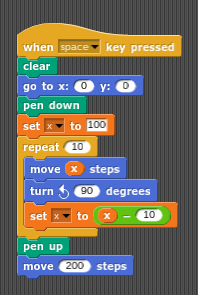
\includegraphics{spiral.png}
\end{center}
giving a spiral
\begin{center}
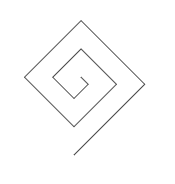
\includegraphics{spiral_pic.png}
\end{center}
Try modifying your programme in the same way so that you get smaller and smaller squares retreating into one corner, like this
\begin{center}
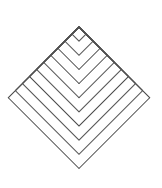
\includegraphics{repeat_squares_pic.png}
\end{center}
so
\begin{center}
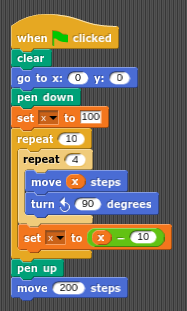
\includegraphics{repeat_squares.png}
\end{center}
If you want to you can try playing with you program a bit to give other patterns, like this
\begin{center}
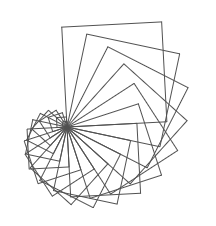
\includegraphics{squares_spiral_pic.png}
\end{center}
so 
\begin{center}
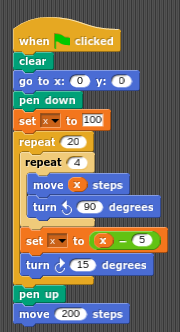
\includegraphics{squares_spiral.png}
\end{center}
Try modifying your circle programme to draw a round spiral.
\begin{center}
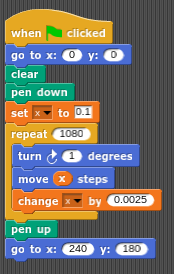
\includegraphics{circle_spiral.png}
\end{center}


This next programme draws a star;

This next programme draws a star
\begin{center}
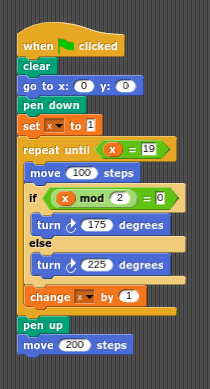
\includegraphics{star.png}
\end{center}

You can mess with programme a bit, maybe changing the angles or putting the whole thing in a loop to give something like this
\begin{center}

\includegraphics{rotating_star_pic.png}
\end{center}
so
\begin{center}
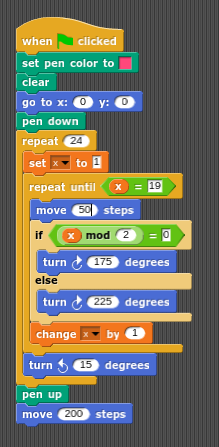
\includegraphics{rotating_star.png}
\end{center}


Imagine you want to use the same commands a few times; in this
programme for example we draw a square, move over a bit and draw
another:
\begin{center}
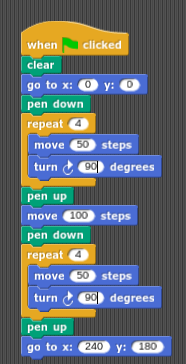
\includegraphics{two_squares.png}
\end{center}
Here we will make a block called square that draws a square: the block
commands are at the bottom of the variable menu:
\begin{center}
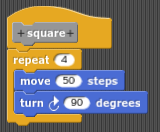
\includegraphics{two_squares_block_block.png}
\end{center}
This block draws a square, so our two square code becomes a bit
neater, quicker to input and easier to read:
\begin{center}
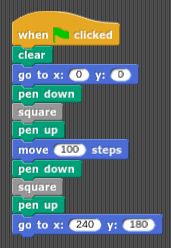
\includegraphics{two_squares_block.png}
\end{center}
You can make your blocks more flexible by adding \textsl{arguments};
these are variables that work inside the block that you can send from
the main programme, you make them by clicking the plus by the block
name.
\begin{center}
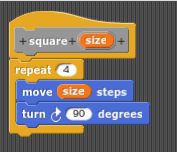
\includegraphics{two_squares_block_size_block.png}
\end{center}
and
\begin{center}
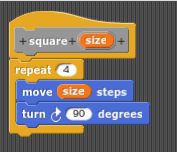
\includegraphics{two_squares_block_size_block.png}
\end{center}
draws the two squares different sizes.
 Try rewriting your original shrinking square code with blocks.
\begin{center}
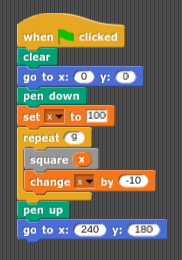
\includegraphics{shrinking_square_block.png}
\end{center}

If they finish this, maybe try recursion:
\begin{center}
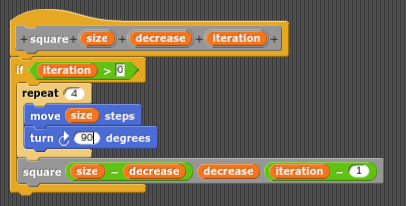
\includegraphics{shrinking_square_recursion_block.png}
\end{center}
draws the two squares different sizes.  Try rewriting your original
shrinking square code with blocks.
\begin{center}
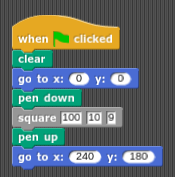
\includegraphics{shrinking_square_recursion.png}
\end{center}

Try writing a block to make a circle with the radius as the argument
\begin{center}
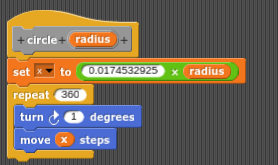
\includegraphics{circle_block.png}
\end{center}
Can you improve your circle block so that you also send the $x$ and $y$ location of the center of the circle?
\begin{center}
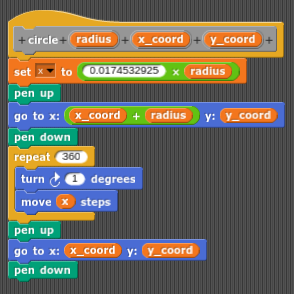
\includegraphics{centre_circle_block.png}
\end{center}

If anyone is finished with all of this maybe go on to this
\begin{center}
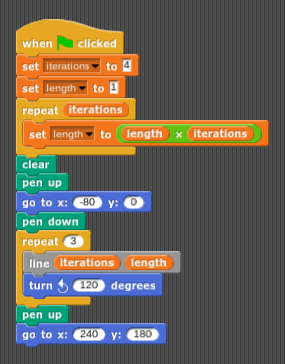
\includegraphics{koch.png}
\end{center}
with block
\begin{center}
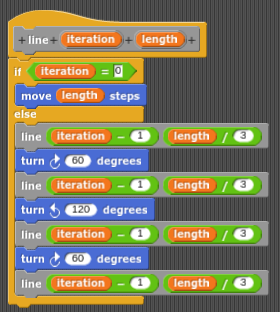
\includegraphics{koch_block.png}
\end{center}
draws
\begin{center}
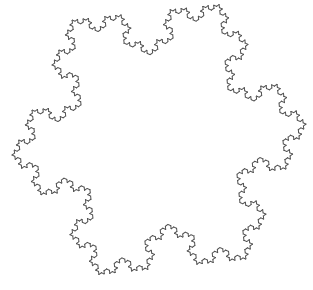
\includegraphics{koch_pic.png}
\end{center}



\end{document}
